\chapter{Generative models}

\begin{description}
    \item[Generative model] \marginnote{Generative model}
        Model that tries to learn a probability distribution $p_\text{model}$ close to that of the data $p_\text{data}$.

        This can be done either by:
        \begin{itemize}
            \item Explicitly estimating the distribution.
            \item Building a generator to sample data from the distribution $p_\text{model}$ and possibly providing a likelihood.
        \end{itemize}

        \begin{remark}
            Generative models are suited for problems with multi-modal outputs (i.e. with no unique solution).
        \end{remark}

    \item[Latent variable model] \marginnote{Latent variable model}
        Given a vector of values $z$ with known prior distribution $P(z)$,
        a latent variable model expresses the probability of a data point $X$ (of the visible space) through marginalization over $z$:
        \[ P(X) = \int P(X|z) P(z) \,dz \approx \mathbb{E}_{z \sim P(z)} P(X|z) \]
        $z$ is considered the latent encoding of $X$ (usually it is some sort of noise).

        The network (generator) on input $z$ can either learn:
        \begin{itemize}
            \item The probability $P(X|z)$.
            \item To generate data points $\hat{X}$ (most likely) belonging to the distribution $P(X|z)$.
        \end{itemize} 

        \begin{figure}[H]
            \centering
            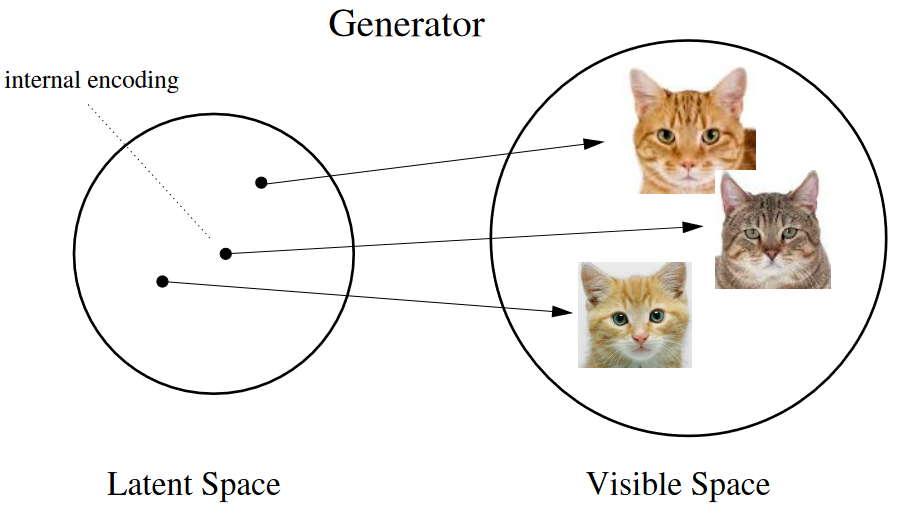
\includegraphics[width=0.45\linewidth]{./img/latent_space.png}
        \end{figure}
\end{description}

Generative models are categorized into two families:
\begin{descriptionlist}
    \item[Compressive models] \marginnote{Compressive models}
        Models where the latent space is smaller than the visible space.

    \item[Dimension-preserving models] \marginnote{Dimension-preserving models}
        Models where the latent space has the same dimension as the visible space.
\end{descriptionlist}

\begin{remark}
    Training latent variable models requires a way to encode the visible training data $X$ into their latent space $z$.
    Training relying only on the latent space does not make sense as, in this case, the output of the generator can be arbitrary.
\end{remark}



\section{Variational autoencoder (VAE)}
\marginnote{Variational autoencoder (VAE)}

Approach belonging to the family of compressive models.


\subsection{Training}

An autoencoder is modified in such a way that:
\begin{itemize}
    \item The encoder takes as input a visible data point $X$ and outputs its latent encoding $z$.
        The encoder is trained to force the marginal distribution of the latent space $Q(z) = \mathbb{E}_{X \sim P_\text{data} Q(z|X)}$ 
        into a known distribution (usually a standard Gaussian).

    \item The decoder (generator) takes as input the latent encoding $z$ of the encoder and outputs a reconstruction $\hat{X}$.
\end{itemize}

\begin{figure}[H]
    \centering
    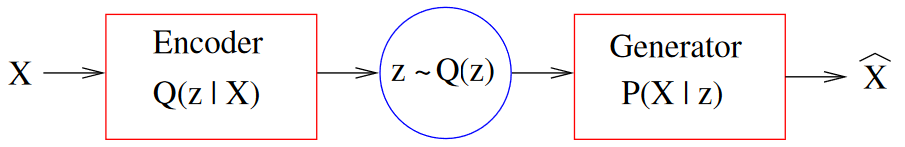
\includegraphics[width=0.5\linewidth]{./img/vae.png}
\end{figure}

It is assumed that for each different input $X$, $Q(z|X)$ has a different Gaussian distribution $G(\mu(X), \sigma(X))$
where both $\mu(X)$ and $\sigma(X)$ are computed by the encoder.

$z=\mu(X)$ can be seen as the latent encoding of $X$, 
while $\sigma(X)$ represents an area of the latent space around $z$ that encodes an information similar to $X$.

During training, the decoder receives in input a point sampled around $\mu(X)$ with variance $\sigma(X)$.

Two losses are used:
\begin{descriptionlist}
    \item[Reconstruction distance] 
        Aims to minimize the distance between the input $X$ and its reconstruction $\hat{X}$:
        \[ \Vert X - \hat{X} \Vert^2 \]

    \item[Kullback-Leibler divergence] 
        Aims to bring the marginal inference distribution $Q(z)$ close to a known distribution (e.g. a standard Gaussian):
        \[ \text{KL}[ Q(z | X) || P(z) ] = \text{KL}[ Q(z | X) || \mathcal{N}(0, 1) ] \]

        \begin{remark}
            The loss is applied to the single distributions $Q(z | X)$ but the effects are propagated to the marginal $Q(z)$.
        \end{remark}

        \begin{remark}
            An effect of this loss (with the standard Gaussian) is to:
            \begin{itemize}
                \item Push $\mu(X)$ towards 0 (i.e. occupying a small area of the latent space).
                \item Push $\sigma(X)$ towards 1 (i.e. making the latent variables have a larger coverage space to make it easier to generate new significant data).
            \end{itemize}
            \begin{figure}[H]
                \centering
                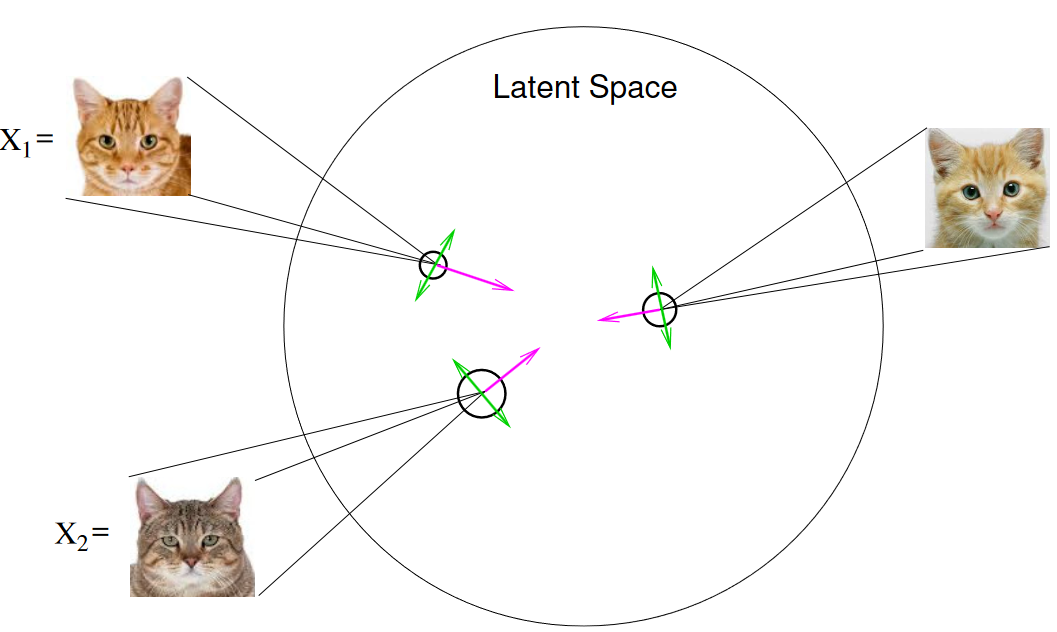
\includegraphics[width=0.4\linewidth]{./img/kl_vae.png}
                \caption{Effect of the KL-divergence on the latent space}
            \end{figure}
        \end{remark}
\end{descriptionlist}

\begin{figure}[H]
    \centering
    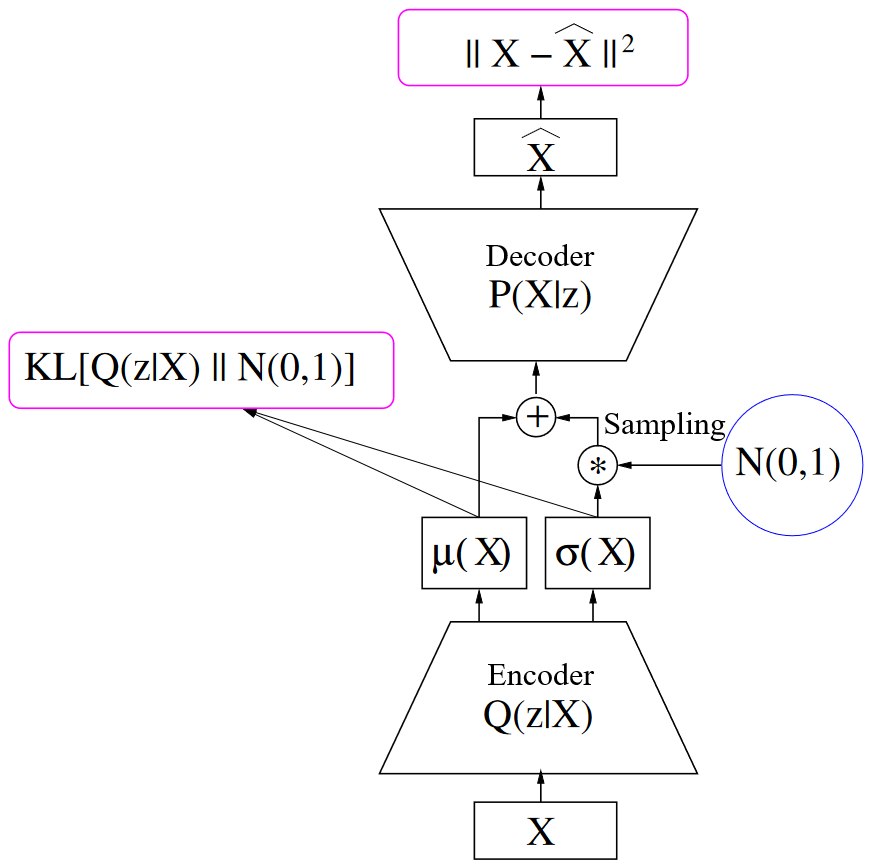
\includegraphics[width=0.4\linewidth]{./img/vae_training.png}
    \caption{Recap of the VAE training process}
\end{figure}



\subsection{Inference}

During inference, the encoder is not used as there are no visible input data $X$.
The decoder generates new data by simply taking as input a latent variable $z$ sampled from its prior distribution (e.g. a standard Gaussian).



\subsection{Problems}

\begin{itemize}
    \item Balancing the two losses is difficult.
    \item It is subject to the posterior collapse problem, where the model learns to ignore a subset of latent variables.
    \item There might be a mismatch between the prior distribution and the learned latent distribution.
    \item Generated images are blurry.
\end{itemize}



\section{Generative adversarial network (GAN)}
\marginnote{Generative adversarial network (GAN)}

Approach belonging to the family of compressive models.

\subsection{Training}
During training, the generator $G$ is paired with a discriminator $D$ that learns to distinguish between real and generated data.

The loss function is the following:
\[
    \mathcal{V}(D, G) = \mathbb{E}_{x \sim p_\text{data}(x)}[\log D(x)] + \mathbb{E}_{z \sim p_z(z)}[\log\big( 1 - D(G(z)) \big)]
\]
where:
\begin{itemize}
    \item $\mathbb{E}_{x \sim p_\text{data}(x)}[\log D(x)]$ is the negative cross-entropy of the discriminator w.r.t. the true data distribution $p_\text{data}$
        (i.e. how well the discriminator recognizes real data).
    \item $\mathbb{E}_{z \sim p_z(z)}[\log\big( 1 - D(G(z)) \big)]$ is the negative cross-entropy of the discriminator w.r.t. the generator
        (i.e. how well the discriminator is able to detect the generator).
\end{itemize}
In other words, the loss aims to:
\begin{itemize}
    \item Instruct the discriminator to spot the generator ($\max_D \mathcal{V}(D, G)$).
    \item Instruct the generator to fool the discriminator ($\min_G \mathcal{V}(D, G)$).
\end{itemize}

\begin{figure}[H]
    \centering
    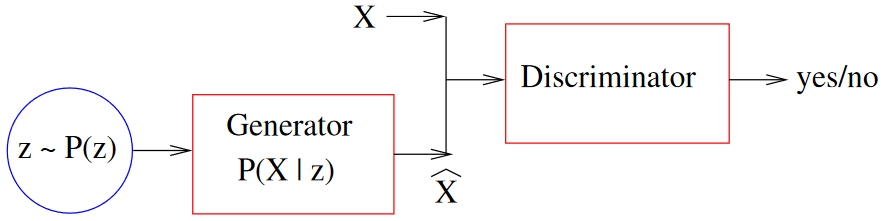
\includegraphics[width=0.5\linewidth]{./img/gan.png}
\end{figure}

For more stability, training is done alternately by training the discriminator with the generator frozen and vice versa.

\begin{remark}
    GANs have the property of pushing the reconstruction towards the natural image manifold.
    \begin{figure}[H]
        \centering
        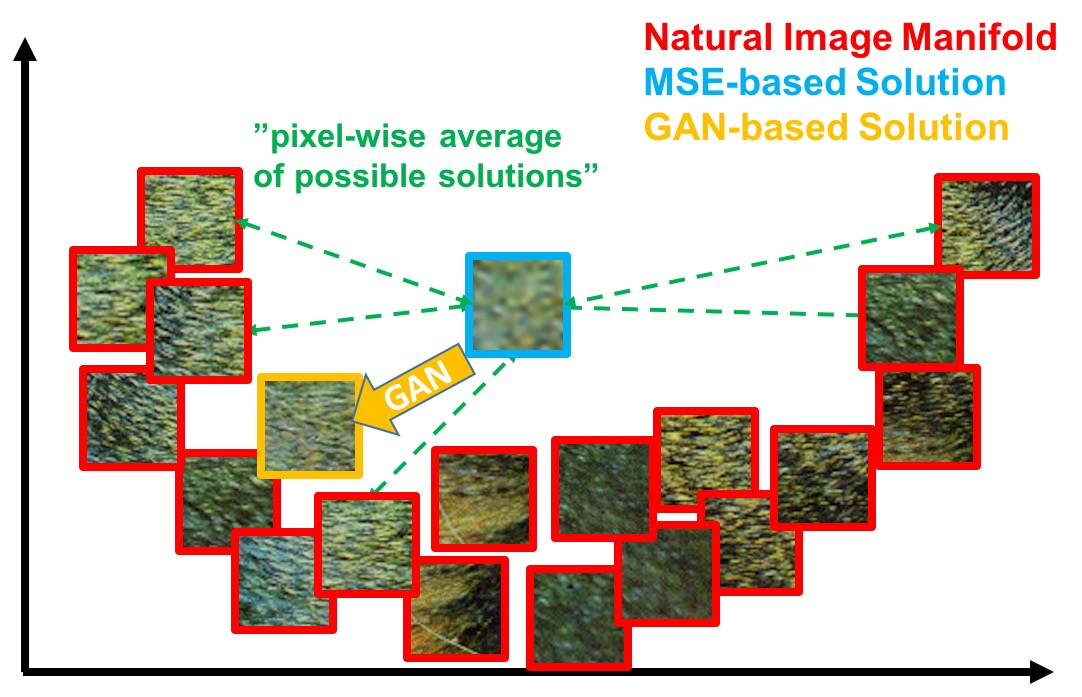
\includegraphics[width=0.4\linewidth]{./img/gan_manifold.png}
        \caption{Comparison of GAN and MSE generated images. MSE is obtained as the pixel-wise average of the natural images.}
    \end{figure}
\end{remark}


\subsection{Problems}

\begin{itemize}
    \item A generator able to fool the discriminator does not necessarily mean that the generated images are good.
    \item There are problems related to counting, perspective and global structure.
    \item The generator tends to specialize on fixed samples (mode collapse).
\end{itemize}



\section{Normalizing flows}
\marginnote{Normalizing flows}

Approach belonging to the family of dimension-preserving models.

The generator is split into a chain of invertible transformations.
During training, the log-likelihood is maximized.

\begin{remark}
    Using only invertible transformations limits the expressiveness of the model.
\end{remark}

\begin{figure}[H]
    \centering
    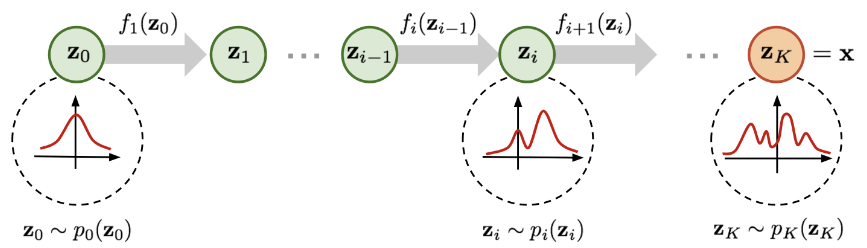
\includegraphics[width=0.65\linewidth]{./img/normalizing_flow.png}
\end{figure}



\section{Diffusion model}
\marginnote{Diffusion model}

Approach belonging to the family of dimension-preserving models.


\subsection{Training (forward diffusion process)}

Given an image $x_0$ and a signal ratio $\alpha_t$ (that indicates how much original data is in the noisy image),
the generator $G$ is considered as a denoiser and a training step $t$ does the following:
\begin{enumerate}
    \item Normalize $x_0$.
    \item Generate a Gaussian noise $\varepsilon \sim \mathcal{N}(0, 1)$.
    \item Generate a noisy version $x_t$ of $x_0$ by injecting the noise as follows:
        \[ x_t = \sqrt{\alpha_t} \cdot x_0 + \sqrt{1-\alpha_t} \cdot \varepsilon \]
    \item Make the network predict the noise $G(x_t, \alpha_t)$ and train it to minimize the prediction error:
        \[ \Vert \varepsilon - G(x_t, \alpha_t) \Vert \]
\end{enumerate}

\begin{remark}
    The values of $\alpha_t$ are fixed by a scheduler.
\end{remark}


\subsection{Inference (reverse diffusion process)}

The generation process is split into a finite chain of $T$ denoising steps that attempt to remove a Gaussian noise with varying $\sigma$.
(i.e. it is assumed that the latent space is a noisy version of the image).

Given a generator $G$ and a fixed signal ratio scheduling $\alpha_T > \dots > \alpha_1$, an image is sampled as follows:
\begin{enumerate}
    \item Start from some random noise $x_T \sim \mathcal{N}(0, 1)$.
    \item For $t$ in $T, \dots, 1$:
    \begin{enumerate}
        \item Estimate the noise using the generator $G(x_t, \alpha_t)$.
        \item Compute the denoised image $\hat{x}_0$:
            \[ \hat{x}_0 = \frac{x_t - \sqrt{1-\alpha_t} \cdot G(x_t, \alpha_t)}{\sqrt{\alpha_t}} \]
        \item Compute a new noisy image for the next iteration by re-injecting some noise with signal ratio $\alpha_{t-1}$ (i.e. inject an amount of noise that is less than this iteration):
            \[ x_{t-1} = \sqrt{\alpha_{t-1}} \cdot \hat{x}_0 + \sqrt{1 - \alpha_{t-1}} \cdot \varepsilon \]
    \end{enumerate}
\end{enumerate}

\begin{figure}[H]
    \centering
    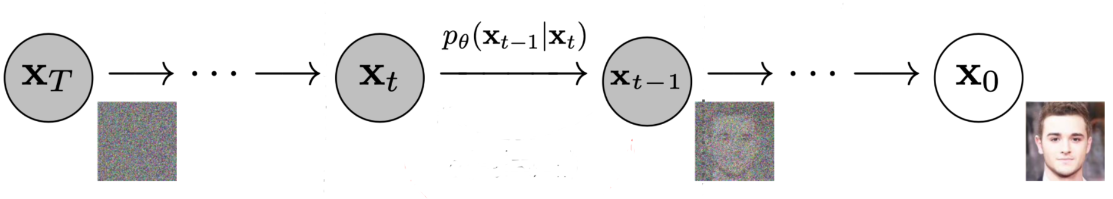
\includegraphics[width=0.65\linewidth]{./img/diffusion_model.png}
\end{figure}

\begin{remark}
    A conditional U-net for denoising works well as the generator.
\end{remark}



\section{Latent space exploration}

\begin{description}
    \item[Representation learning] \marginnote{Representation learning}
        Learning a latent space in such a way that particular changes reflect a desired alteration of the visible space.

        \begin{remark}
            Real-world data depend on a relatively small set of latent features.
        \end{remark}

    \item[Disentanglement] \marginnote{Disentanglement}
        The latent space learned by a model is usually entangled (i.e. a change in one attribute might affect the others).

        Through linear maps, it is possible to pass from one latent space to another.
        This can be done by finding a small set of points common to the starting and destination spaces (support set)
        and defining a map based on those points.

        \begin{remark}
            The latent space seems to be independent of:
            \begin{itemize}
                \item The training process.
                \item The training architecture.
                \item The learning objective (i.e. GAN and VAE might have the same latent space).
            \end{itemize}
        \end{remark}

        \begin{figure}[H]
            \centering
            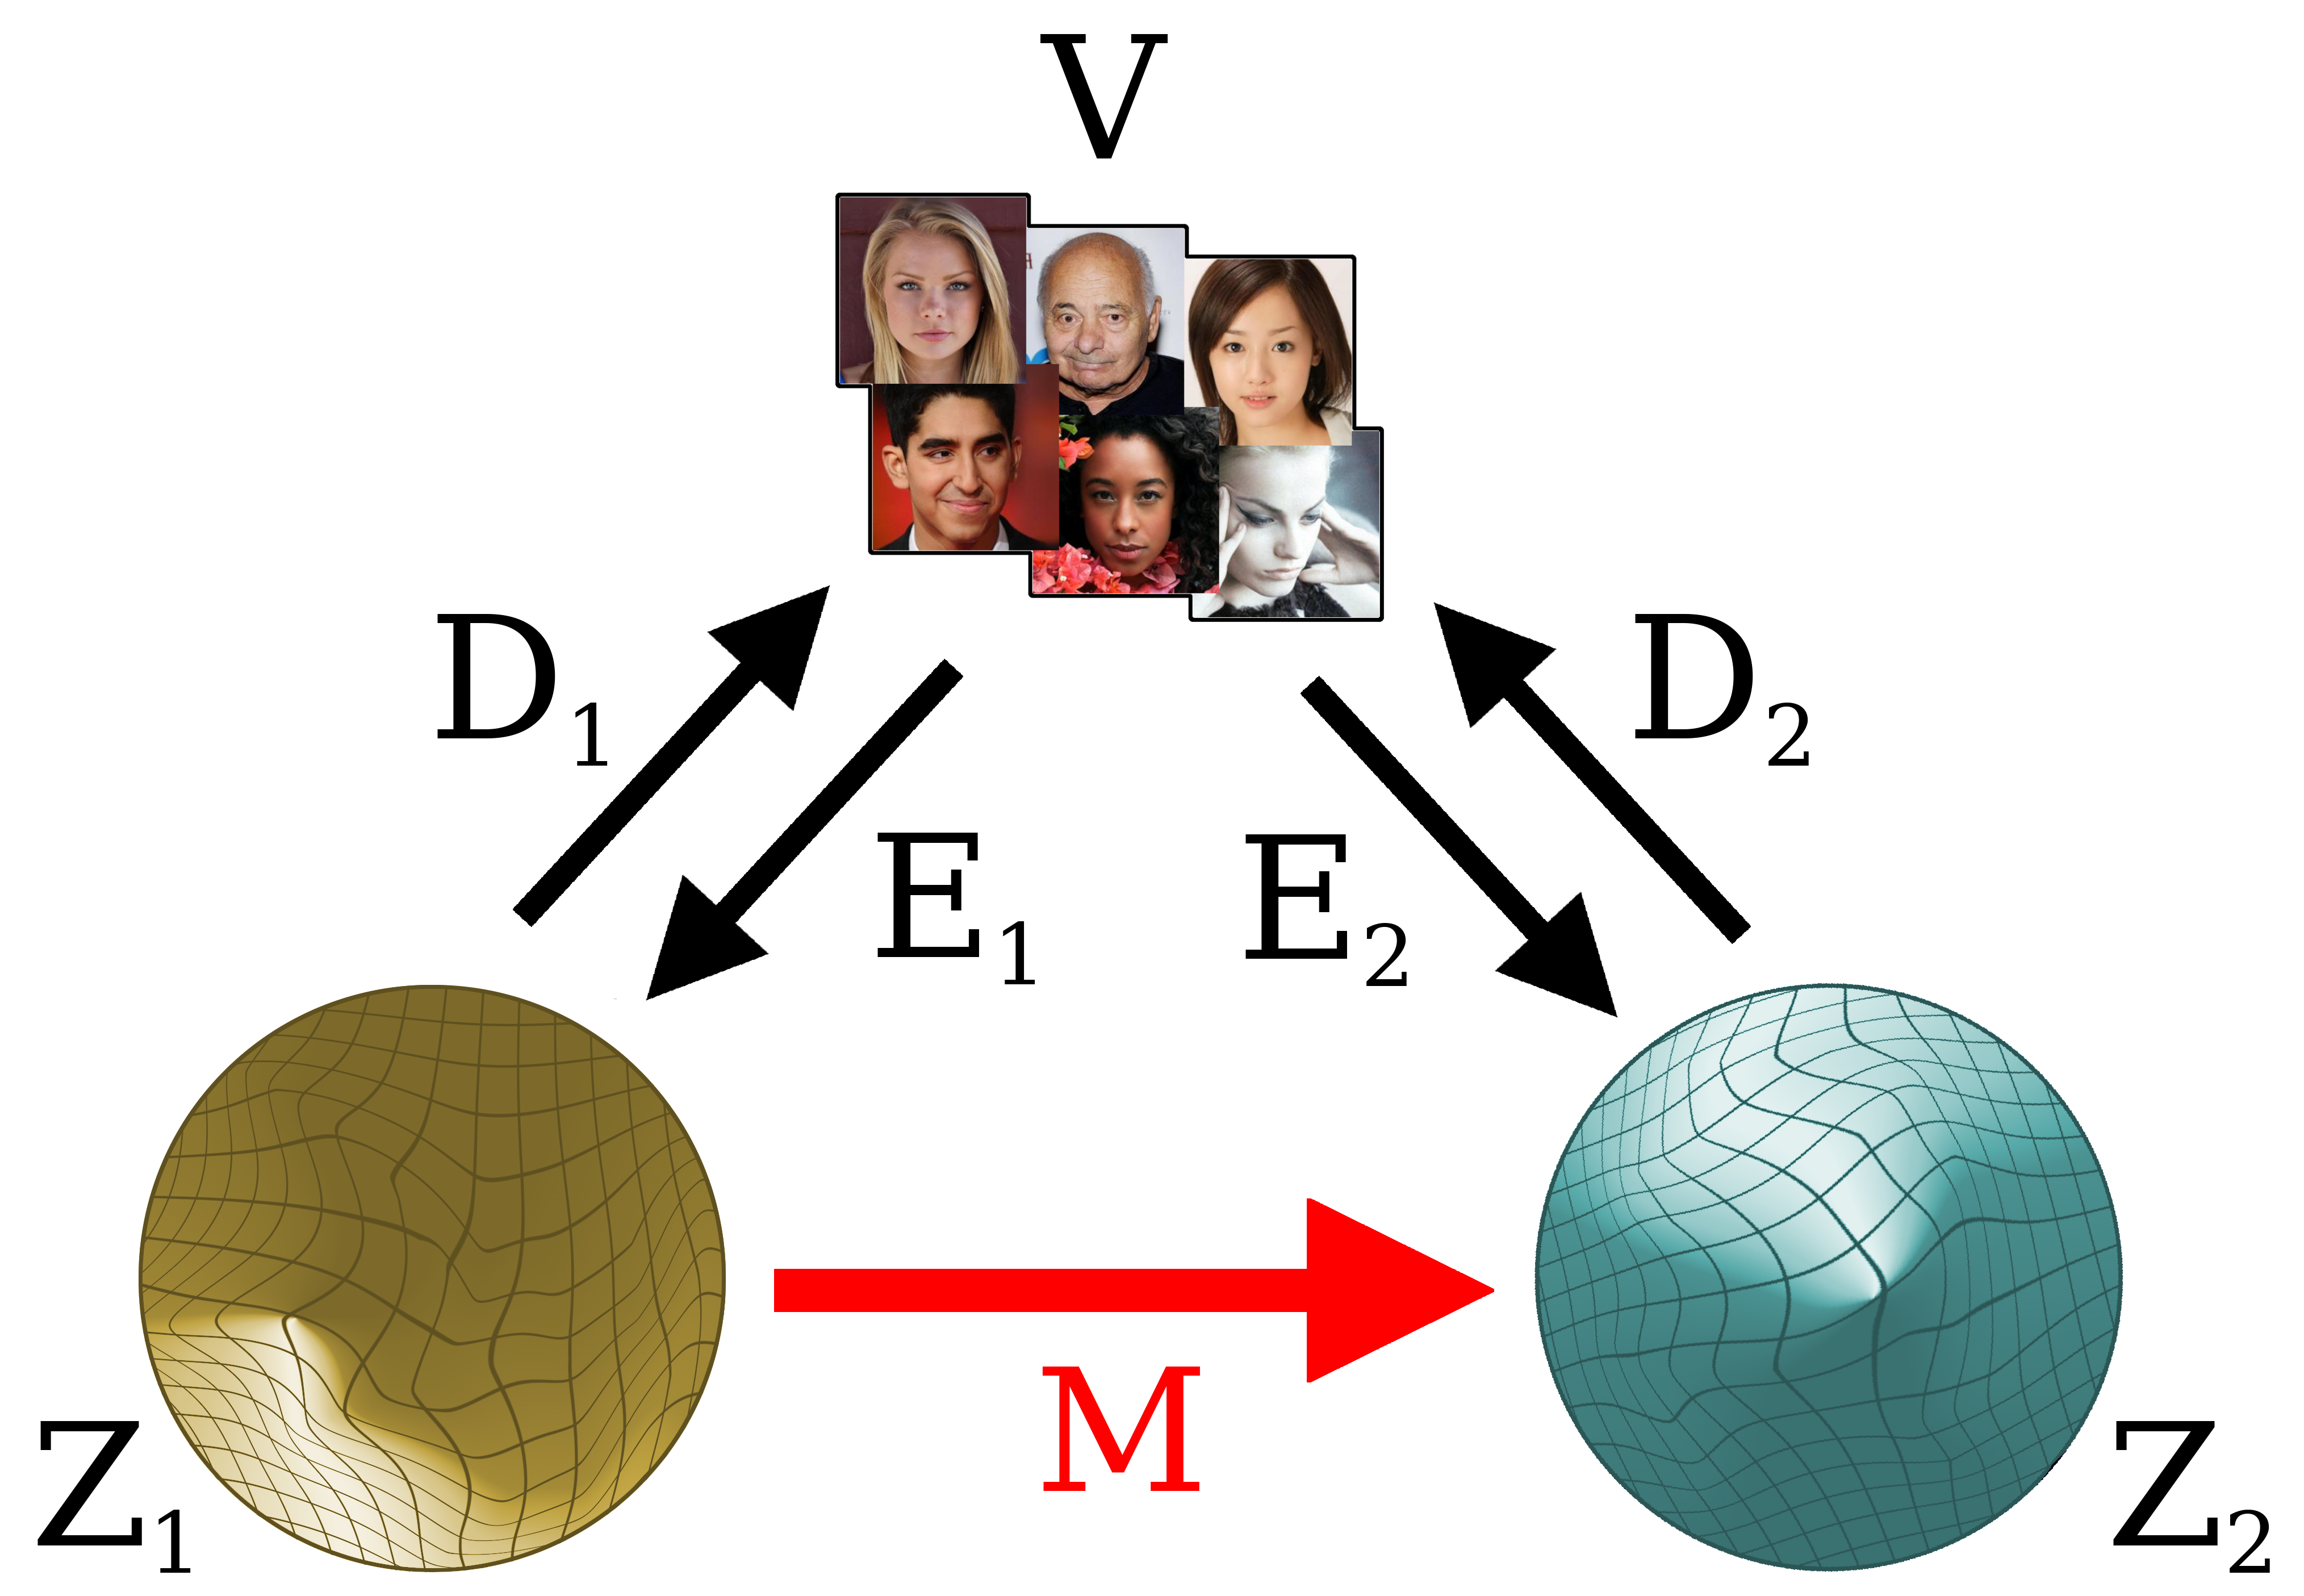
\includegraphics[width=0.3\linewidth]{./img/latent_mapping.png}
            \caption{
                \parbox[t]{0.72\linewidth}{
                    Example of mapping from a latent space $Z_1$ to a space $Z_2$ through $M$.
                    The two spaces are evaluated on the visible space $V$.
                }
            }
        \end{figure}
\end{description}